\chapter{Results} \label{chap_results}

The architecture described in Chapter \ref{chap_results} was fully implemented and tested in simulation, but unfortunately it was not tested on actual hardware. But assuming that the module it feed data every clock cycle we can calculate the theoretical performance to be 

\begin{equation} \label{eq_theoretical_performance}
\frac{f}{I\times(n \times n) + (k \times k) + 5} ~Conv\_layer\_op/s
\end{equation}

Where \textit{f} is the clock frequency, \textit{I} is the number input images, \textit{n} is the image dimension, \text{k} is the kernel dimension, and the 5 is the depth of the pipeline. \textit{Conv\_layer\_op/s} is the number of times the full computation of the convolution layer can be done per second. That is convoluting all the images \textit{I}, apply the sigmoid function, and subsample/max-pooling the result. 

Using Equation \ref{eq_theoretical_performance} the Imagezor architecture was  compared  to a Intel Core i5-450. The CPU executed a C program which performed all the operations of the convolution layer. In order to compare the scalability both different images sizes and kernel sizes was tested. The results from the simulation is shown in Figure \ref{fig_cpu_cmp_results}.
\begin{figure}
  \centering
      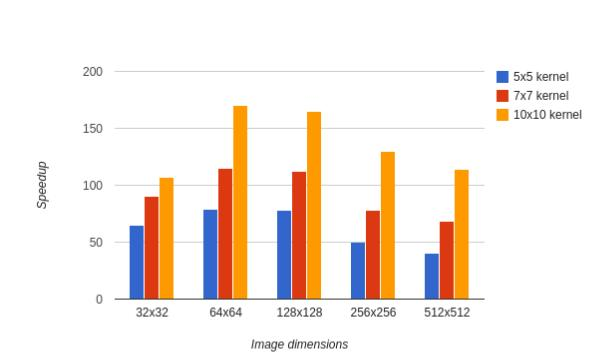
\includegraphics[width=0.6\textwidth]{Figures/Results/Speedup_chart}
  \caption{The theoretical speedup our module had compared to a CPU.}
  \label{fig_cpu_cmp_results}
\end{figure}

As can be seen by the figure, Imagezor is up to 170x faster than the CPU, and uses only a fraction of the power.  

\textbf{If time permits, write a GPU implementation to compare against.}

